% Uebung Leistungsberechnung  nach Brinkmeyer
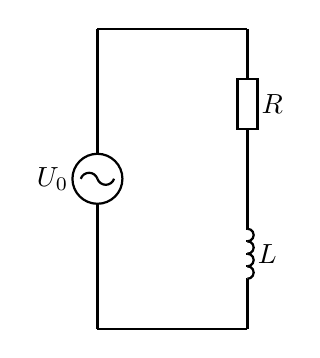
\begin{tikzpicture}[scale=2.54]%
% dpic version 2024.01.01 option -g for TikZ and PGF 1.01
\ifx\dpiclw\undefined\newdimen\dpiclw\fi
\global\def\dpicdraw{\draw[line width=\dpiclw]}
\global\def\dpicstop{;}
\dpiclw=0.8bp
\dpiclw=0.8bp
\dpicdraw (0,0)
 --(0,-0.625)\dpicstop
\dpicdraw (0,-0.75) circle (0.049213in)\dpicstop
\dpicdraw (-0,-0.75)
 ..controls (-0.005978,-0.732065) and (-0.022762,-0.719968)
 ..(-0.041667,-0.719968)
 ..controls (-0.060571,-0.719968) and (-0.077355,-0.732065)
 ..(-0.083333,-0.75)\dpicstop
\dpicdraw (0,-0.75)
 ..controls (0.005978,-0.767935) and (0.022762,-0.780032)
 ..(0.041667,-0.780032)
 ..controls (0.060571,-0.780032) and (0.077355,-0.767935)
 ..(0.083333,-0.75)\dpicstop
\dpicdraw (0,-0.875)
 --(0,-1.5)\dpicstop
\draw (-0.125,-0.75) node[left=-2bp]{$ U_0$};
\dpicdraw (0,0)
 --(0.75,0)\dpicstop
\dpicdraw (0.75,0)
 --(0.75,-0.25)\dpicstop
\dpicdraw (0.75,-0.5)
 --(0.8,-0.5)
 --(0.8,-0.25)
 --(0.7,-0.25)
 --(0.7,-0.5)
 --(0.75,-0.5)\dpicstop
\dpicdraw (0.75,-0.5)
 --(0.75,-0.75)\dpicstop
\draw (0.8,-0.375) node[right=-2bp]{$ R$};
\dpicdraw (0.75,-0.75)
 --(0.75,-1)\dpicstop
\dpicdraw (0.75,-1)
 --(0.744444,-1)\dpicstop
\dpicdraw (0.75,-1)
 ..controls (0.761165,-1) and (0.771481,-1.005956)
 ..(0.777063,-1.015625)
 ..controls (0.782646,-1.025294) and (0.782646,-1.037206)
 ..(0.777063,-1.046875)
 ..controls (0.771481,-1.056544) and (0.761165,-1.0625)
 ..(0.75,-1.0625)\dpicstop
\dpicdraw (0.75,-1.0625)
 --(0.744444,-1.0625)\dpicstop
\dpicdraw (0.75,-1.0625)
 ..controls (0.761165,-1.0625) and (0.771481,-1.068456)
 ..(0.777063,-1.078125)
 ..controls (0.782646,-1.087794) and (0.782646,-1.099706)
 ..(0.777063,-1.109375)
 ..controls (0.771481,-1.119044) and (0.761165,-1.125)
 ..(0.75,-1.125)\dpicstop
\dpicdraw (0.75,-1.125)
 --(0.744444,-1.125)\dpicstop
\dpicdraw (0.75,-1.125)
 ..controls (0.761165,-1.125) and (0.771481,-1.130956)
 ..(0.777063,-1.140625)
 ..controls (0.782646,-1.150294) and (0.782646,-1.162206)
 ..(0.777063,-1.171875)
 ..controls (0.771481,-1.181544) and (0.761165,-1.1875)
 ..(0.75,-1.1875)\dpicstop
\dpicdraw (0.75,-1.1875)
 --(0.744444,-1.1875)\dpicstop
\dpicdraw (0.75,-1.1875)
 ..controls (0.761165,-1.1875) and (0.771481,-1.193456)
 ..(0.777063,-1.203125)
 ..controls (0.782646,-1.212794) and (0.782646,-1.224706)
 ..(0.777063,-1.234375)
 ..controls (0.771481,-1.244044) and (0.761165,-1.25)
 ..(0.75,-1.25)\dpicstop
\dpicdraw (0.75,-1.25)
 --(0.744444,-1.25)\dpicstop
\dpicdraw (0.75,-1.25)
 --(0.75,-1.5)\dpicstop
\draw (0.78125,-1.125) node[right=-2bp]{$ L$};
\dpicdraw (0.75,-1.5)
 --(0,-1.5)\dpicstop
\end{tikzpicture}%
